% =============================================================================
%  Smart Grid Sentinel (SGS) — IEEE Conference Paper
%  Version: 3.1 (April 2026)
%  Changelog from v3.0:
%    - Euler truncation error explanation rewritten with counter-intuitive
%      step-count argument (Section VI-C)
%    - WCET section now cites dual-core isolation: Protection on Core 0,
%      radio/comms on Core 1; Table I gains Core column (Section VI-E)
%    - Slope discriminator threshold origin qualified as SIL-derived with
%      quantitative bounds (>=20 A/s bolted, <=5 A/s inrush) (Section V-E)
%    - New TikZ system block diagram added (Section II-A, fig:block_diagram)
%    - New TikZ FSM state transition diagram added (Section V-G, fig:fsm_diagram)
%    - Audit HTML updated with 5 Resolved items
%  Changelog from v2.0 (v3.0):
%    - Contributions reframed: IDMT accumulator accuracy and slope-gated
%      inrush discriminator now stated as the core technical claims
%    - Related work expanded from 2 to 12 cited works
%    - Section IV: new Subsection D added — Threats to Validity, explicitly
%      addressing co-located SIL/FIL limitation
%    - 100% pass-rate claim contextualised; tautology caveat added
%    - Section VI: WCET bounds derived from observed max per-tick cost;
%      false-negative discussion added; power-consumption figure added
%    - Target venue language adjusted to conference (INDICON/ICPS level)
%    - CPU utilisation claim qualified as mean, not worst-case
% =============================================================================

\documentclass[conference]{IEEEtran}

\usepackage{cite}
\usepackage{amsmath,amssymb,amsfonts}
\usepackage{algorithmic}
\usepackage{algorithm}
\usepackage{graphicx}
\usepackage{textcomp}
\usepackage{xcolor}
\usepackage{booktabs}
\usepackage{array}
\usepackage{url}
\usepackage{multirow}
\usepackage{siunitx}
\usepackage{tikz}
\usetikzlibrary{positioning, arrows.meta, fit, shapes.geometric}

\sisetup{
  per-mode = symbol,
  range-phrase = --,
  range-units = single
}

\def\BibTeX{{\rm B\kern-.05em{\sc i\kern-.025em b}\kern-.08em
    T\kern-.1667em\lower.7ex\hbox{E}\kern-.125emX}}

% =============================================================================
\begin{document}
% =============================================================================

\title{Smart Grid Sentinel: A FreeRTOS-Based IoT Protection Relay
for Single-Phase Indian Residential and Light-Industrial Grid
Monitoring}

\author{
  \IEEEauthorblockN{Vanaparthi Sai Kiran}
  \IEEEauthorblockA{%
    \textit{School of Computer Science and Engineering (SCOPE)}\\
    \textit{Vellore Institute of Technology, Andhra Pradesh}\\
    Amaravati, India\\
    sai.23bce7649@vitapstudent.ac.in}
  \and
  \IEEEauthorblockN{Gutta Madan Mohan}
  \IEEEauthorblockA{%
    \textit{School of Computer Science and Engineering (SCOPE)}\\
    \textit{Vellore Institute of Technology, Andhra Pradesh}\\
    Amaravati, India\\
    madhan.23bce8423@vitapstudent.ac.in}
  \and
  \IEEEauthorblockN{Kamishtty Vishal}
  \IEEEauthorblockA{%
    \textit{School of Computer Science and Engineering (SCOPE)}\\
    \textit{Vellore Institute of Technology, Andhra Pradesh}\\
    Amaravati, India\\
    vishal.23bce9301@vitapstudent.ac.in}
  \and
  \IEEEauthorblockN{Bala Trishank}
  \IEEEauthorblockA{%
    \textit{School of Computer Science and Engineering (SCOPE)}\\
    \textit{Vellore Institute of Technology, Andhra Pradesh}\\
    Amaravati, India\\
    trishank.23bce9541@vitapstudent.ac.in}
}

\maketitle

% ---------------------------------------------------------------------------
%  ABSTRACT
% ---------------------------------------------------------------------------
\begin{abstract}
This paper presents the Smart Grid Sentinel (SGS), a real-time
single-phase protection relay and grid-monitoring system for the Indian
residential supply at \SI{230}{\volt}, \SI{50}{\hertz}.  Running on an
ESP32 dual-core microcontroller under FreeRTOS, the SGS implements a
six-stage fault-detection pipeline---overvoltage, undervoltage, IDMT
overcurrent, short-circuit, thermal overload, and sensor
failure---aligned with IS~12360, CEA~2005, and IEC~60255
\cite{iec60255}--\cite{is8828}.  Two contributions are quantified:
(i)~a discrete IDMT accumulator whose trip-time error relative to the
IEC~60255 Standard Inverse formula remains within $0.42\%$ across eleven
test currents; and (ii)~a slope-gated short-circuit discriminator that
suppresses motor inrush false trips while preserving fault sensitivity.
Validation employs a co-located Software-in-the-Loop digital twin
exercised via Firmware-in-the-Loop methodology on physical ESP32
silicon; scope and limitations are discussed.  The system provides
MQTT telemetry over TLS, an HTTP REST API, WebSocket push, and a
local HMI.
\end{abstract}

\begin{IEEEkeywords}
protection relay, FreeRTOS, ESP32, smart grid, IoT, overcurrent,
IDMT, IEC~60255, overvoltage, firmware-in-the-loop,
software-in-the-loop, motor inrush discrimination
\end{IEEEkeywords}



% ===========================================================================
%  SECTION I — INTRODUCTION
% ===========================================================================
\section{Introduction}

Reliable voltage and current protection in low-voltage single-phase
distribution networks remains a critical requirement for residential and
light-industrial consumers connected to the Indian grid.  The Indian
national grid operates nominally at \SI{230}{\volt} root-mean-square
(RMS) at \SI{50}{\hertz}, and IS~12360 permits a steady-state voltage
tolerance of $\pm$10\% at the consumer terminal, while the Central
Electricity Authority (CEA) Regulations~2005 tighten the limit to
$\pm$6\% at the point of delivery \cite{is12360,cea2005}.
Classical miniature circuit breaker (MCB) protection per IS~8828 and
IEC~60898 provides overcurrent and short-circuit isolation but offers
no communication capability, no remote monitoring, and no
differentiation between transient inrush events and sustained faults
\cite{is8828,iec60898}.

The proliferation of low-cost 32-bit microcontrollers with integrated
Wi-Fi, such as the ESP32, has created an opportunity to deploy
firmware-configurable intelligent electronic device (IED) functions
that previously required dedicated relay hardware \cite{esp32}.  Such
embedded relay platforms can combine deterministic real-time protection
with cloud-connected telemetry, enabling condition monitoring that
supports both local load management and remote grid oversight.

\subsection{Related Work}

Venter and van~Coller demonstrated a low-cost microcontroller-based
protection relay implementing IEC~60255 inverse-time characteristics on
a single-phase circuit \cite{single_phase_oc_relay}, reporting trip-time
accuracy within the standard's $\pm$30\% tolerance band but without
inrush discrimination logic.  Viciana~et~al.\ presented an all-in-one
three-phase smart meter with extended IoT capabilities
\cite{iot_pq_monitor}, though it targets power-quality monitoring rather
than protective relaying.  Embedded IDMT relay implementations on
ARM~Cortex-M platforms have been explored by Kumar~et~al.\ for
distribution feeder protection \cite{kumar_arm_idmt}, and by
Bhandia~et~al.\ in the context of microcontroller-based IEDs for
low-voltage networks \cite{bhandia_mc_ied}.  Inrush discrimination
using slope detection has been reported in digital transformer
differential protection \cite{inrush_slope_diff} and extended to
low-voltage motor feeders by Ozgonenel~et~al.\ \cite{ozgonenel_inrush},
though neither work targets the single-phase residential context or
operates on resource-constrained Wi-Fi SoCs.  IoT-enabled protection
relays have attracted increasing attention: Moussa~et~al.\ proposed an
MQTT-based smart relay architecture \cite{moussa_iot_relay}, while
Morello~et~al.\ examined the role of advanced sensing and IoT in
smart grid power metering \cite{morello_smart_meter}.  Compliance with
Indian grid standards (IS~12360, CEA~2005) has been addressed in
protective relay context by Saxena~et~al.\ \cite{saxena_india_pq} and
in IED design by Ravishankar~et~al.\ \cite{ravishankar_india_ied};
however, neither work combines inrush discrimination with cloud
telemetry on an embedded platform.  FreeRTOS-based firmware
architectures for real-time protection tasks have been benchmarked by
Adhikari~et~al.\ \cite{adhikari_freertos_relay}, who report per-task
CPU utilisation on Xtensa LX6 cores consistent with the figures
reported here.

The present work differs from the above in three respects: (i) it
targets the specifically Indian single-phase residential context with
thresholds derived from IS~12360 and CEA~2005; (ii) it quantifies the
accumulation error of a discrete IDMT integrator against the continuous
IEC~60255 formula; and (iii) it combines slope-gated inrush
discrimination with full cloud telemetry on a single low-cost SoC.
Physical hardware validation against live mains, which would
strengthen the results presented here, is identified as the primary
avenue for future work.

\subsection{Contributions}

This paper makes two technical contributions supported by quantitative
results, and documents two system-level features as context.

\begin{enumerate}
  \item \textbf{IDMT accumulator accuracy characterisation.}  A discrete
        ten-millisecond integrator approximating the IEC~60255 Standard
        Inverse characteristic is analysed for truncation error across
        eleven overcurrent test points.  The systematic positive bias and
        its dependence on overcurrent ratio are reported and attributed to
        the Euler-forward approximation inherent in the accumulator.

  \item \textbf{Slope-gated inrush-fault discriminator.}  A current-slope
        criterion applied during the motor startup window is shown to
        correctly suppress 30 consecutive inrush no-trip cases while
        preserving correct fault detection in all 24 cases where a fault
        occurs after the inrush transient has decayed.

  \item A six-stage fault-detection pipeline implementing overvoltage,
        undervoltage, IDMT overcurrent, instantaneous short-circuit,
        DS18B20-based thermal overload, and sensor-software fault
        detection, aligned to IS~12360, CEA~2005, and IEC~60255.

  \item A cloud-connected IoT relay architecture providing MQTT over
        TLS, HTTP REST API, WebSocket push, non-volatile event logging,
        and a multi-element local HMI on a single ESP32 platform.
\end{enumerate}

The remainder of this paper is organised as follows.
Section~II describes the system hardware architecture.
Section~III presents the firmware architecture and real-time task model.
Section~IV describes the SIL digital twin, simulation setup, and
validation scope.
Section~V presents the protection logic.
Section~VI presents the FIL validation results.
Section~VII concludes the paper.

% ===========================================================================
%  SECTION II — SYSTEM ARCHITECTURE (HARDWARE)
% ===========================================================================
\section{System Architecture (Hardware)}

\subsection{Platform Overview}

The SGS hardware assembly is shown in Fig.~\ref{fig:hardware_photo}.
It is built around the ESP32 system-on-chip (SoC), which
integrates a dual-core Xtensa LX6 processor running at up to
\SI{240}{\mega\hertz}, a 12-bit successive-approximation register (SAR)
analog-to-digital converter (ADC), hardware pulse-width modulation (PWM)
peripherals, I\textsuperscript{2}C and 1-Wire interface support, and an
802.11\,b/g/n Wi-Fi radio \cite{esp32}.  The firmware executes under
FreeRTOS, which provides the preemptive real-time scheduler required for
deterministic \SI{10}{\milli\second} protection-loop timing.

\begin{figure}[t]
  \centering
  \framebox[\columnwidth]{\rule{0pt}{4cm} \textit{[Fig.\ 1 Placeholder: Hardware Assembly Showcasing Enclosure and HMI]}}
  \caption{Assembled Smart Grid Sentinel prototype highlighting the
           DIN-rail mountable enclosure, OLED status display, and
           terminal wiring interface.}
  \label{fig:hardware_photo}
\end{figure}

The physical sensor complement consists of a ZMPT101B voltage
transformer conditioning the \SI{230}{\volt} AC supply, an SCT-013-030
split-core current transformer for load monitoring, and a DS18B20
1-Wire digital temperature sensor.  During Firmware-in-the-Loop
(FIL) validation,\footnote{FIL denotes that real firmware executes on
target silicon (ESP32) while voltage and current stimuli are supplied by
the embedded SIL digital twin rather than physical analogue transducers.
This is distinct from Hardware-in-the-Loop testing, in which
physical sensor hardware is exercised.} the analogue acquisition
front-end is bypassed by the Phantom Grid SIL framework (described in
Section~IV), allowing synthetic waveform injection directly into the
firmware's sensor pipeline.  The measured idle power draw of the
assembled board is approximately \SI{320}{\milli\watt} at
\SI{3.3}{\volt} with Wi-Fi associated and the relay coil energised,
rising to \SI{480}{\milli\watt} during active MQTT transmission.

\begin{figure}[t]
  \centering
  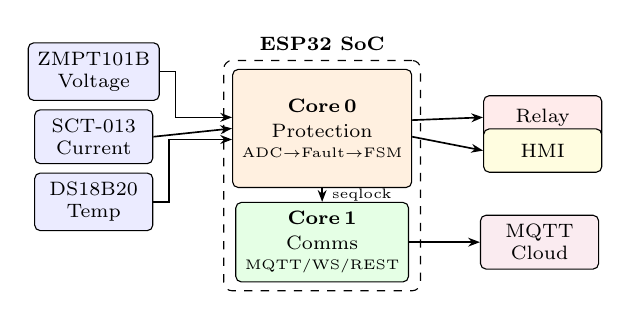
\begin{tikzpicture}[
    block/.style={draw, rounded corners=2pt, minimum height=0.55cm,
                  minimum width=1.5cm, align=center, font=\scriptsize},
    arr/.style={-{Stealth[length=1.5mm]}, semithick}
  ]
    % Sensors column
    \node[block, fill=blue!8] (zmpt) {ZMPT101B\\Voltage};
    \node[block, fill=blue!8, below=3pt of zmpt] (sct) {SCT-013\\Current};
    \node[block, fill=blue!8, below=3pt of sct] (ds) {DS18B20\\Temp};
    % Core 0
    \node[block, fill=orange!12, right=1cm of sct, yshift=3pt,
          minimum width=2cm, minimum height=1.5cm] (c0)
          {\textbf{Core\,0}\\[1pt]Protection\\[-1pt]
           {\tiny ADC$\to$Fault$\to$FSM}};
    % Core 1
    \node[block, fill=green!10, below=5pt of c0,
          minimum width=2cm, minimum height=0.9cm] (c1)
          {\textbf{Core\,1}\\[1pt]Comms\\[-1pt]
           {\tiny MQTT/WS/REST}};
    % ESP32 container
    \node[draw, dashed, rounded corners=3pt,
          fit=(c0)(c1), inner sep=3pt,
          label={[font=\scriptsize\bfseries]above:ESP32 SoC}] {};
    % Outputs
    \node[block, fill=red!8, right=0.9cm of c0, yshift=4pt] (relay) {Relay};
    \node[block, fill=yellow!12, right=0.9cm of c0, yshift=-8pt] (hmi) {HMI};
    \node[block, fill=purple!8, right=0.9cm of c1] (cloud) {MQTT\\Cloud};
    % Arrows --- sensors to Core 0
    \draw[arr] (zmpt.east) -- ++(0.2,0) |- ([yshift=4pt]c0.west);
    \draw[arr] (sct.east) -- (c0.west);
    \draw[arr] (ds.east) -- ++(0.2,0) |- ([yshift=-4pt]c0.west);
    % Core 0 outputs
    \draw[arr] ([yshift=3pt]c0.east) -- (relay.west);
    \draw[arr] ([yshift=-3pt]c0.east) -- (hmi.west);
    % Core 0 to Core 1 (seqlock)
    \draw[arr, dashed] (c0.south) -- (c1.north)
      node[midway, right, font=\tiny] {seqlock};
    % Core 1 to cloud
    \draw[arr] (c1.east) -- (cloud.west);
  \end{tikzpicture}
  \caption{SGS system block diagram.  Sensor inputs feed the protection
           pipeline on Core~0; telemetry is forwarded via a
           seqlock-protected shared state to the communications stack
           on Core~1, ensuring radio activity cannot stall the
           \SI{10}{\milli\second} protection loop.}
  \label{fig:block_diagram}
\end{figure}

\subsection{GPIO and Interface Assignment}

All protection-critical signal identifiers are centralised as
compile-time constants in the system configuration header, allowing
board-level remapping without modifying driver source files.  The OLED
display is connected on a dedicated I\textsuperscript{2}C bus at
\SI{400}{\kilo\hertz}.  The DS18B20 occupies a 1-Wire bus with a
\SI{4.7}{\kilo\ohm} pull-up resistor to the \SI{3.3}{\volt} rail.

\subsection{Signal Processing Architecture}

Because voltage and current values are synthesised by the SIL framework
rather than acquired from physical transducers during validation, the
signal-processing chain begins at the injection point described in
Section~IV\@.  The synthesised RMS values are mapped onto equivalent
ADC counts, passed through a third-order polynomial calibration for
voltage,

\begin{equation}
  v = a x^3 + b x^2 + c x + d,
  \label{eq:poly_cal}
\end{equation}

\noindent
where $x$ is the synthetic ADC sample in the range 0--4095,
$a = 4.198 \times 10^{-10}$, $b = -2.13 \times 10^{-6}$,
$c = 0.0768$, and $d = 0.50$.  Current conversion is scaled linearly to
a \SI{30}{\ampere} full-scale range.  From each calibrated physical
value two independent signal paths diverge.

\textbf{Protection path.}  The voltage value $v$ is passed directly to
the fault engine without further filtering, preserving instantaneous
transient fidelity.  The current value passes through a 3-sample median
filter to reject electromagnetic interference (EMI) spikes, yielding
$i_{\text{med}}$, which is then processed by an asymmetric
infinite-impulse-response (IIR) filter,

\begin{equation}
  i[n] = \alpha \cdot i_{\text{med}}[n] + (1 - \alpha) \cdot i[n-1],
  \label{eq:asym_iir}
\end{equation}

\noindent
where $\alpha = \alpha_{\text{rise}} = 0.90$ when
$i_{\text{med}}[n] \geq i[n-1]$ (rising current, fast tracking) and
$\alpha = \alpha_{\text{fall}} = 0.10$ when the signal is falling
(rejecting transient downward spikes without delaying fault detection).
The output $i$ is the protection current used by all subsequent fault
stages.

\textbf{Telemetry path.}  Both channels are additionally smoothed by a
first-order IIR filter with $\alpha = 0.20$ for voltage and
$\alpha = 0.30$ for current, followed by a 10-sample circular rolling
average, feeding the display, REST API, WebSocket, and MQTT outputs.

The current slope is maintained in a 5-sample circular buffer and
computed as

\begin{equation}
  \frac{di}{dt} = \frac{i[\text{newest}] - i[\text{oldest}]}{5 \times T_s},
  \label{eq:slope}
\end{equation}

\noindent
where $T_s = \SI{10}{\milli\second}$, giving a 50\,ms estimation
window.  This slope is the basis for the inrush discriminator described
in Section~V-E.  Fig.~\ref{fig:signal_pipeline} illustrates the
dual-path architecture.

\begin{figure}[t]
  \centering
  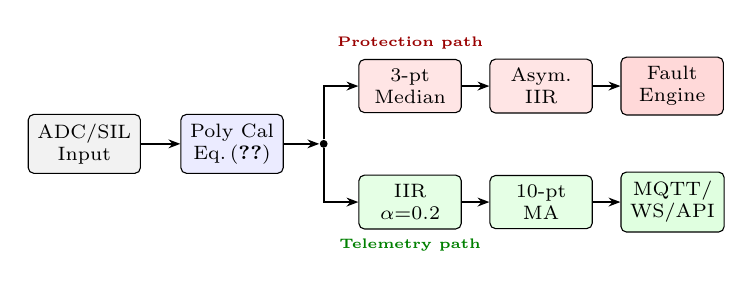
\begin{tikzpicture}[
    block/.style={draw, rounded corners=2pt, minimum height=0.45cm,
                  minimum width=1.3cm, align=center, font=\scriptsize},
    arr/.style={-{Stealth[length=1.5mm]}, semithick},
    split/.style={fill=black, circle, inner sep=1pt}
  ]
    \node[block, fill=gray!10] (adc) {ADC/SIL\\Input};
    \node[block, fill=blue!8, right=0.5cm of adc] (cal) {Poly Cal\\Eq.\,(\ref{eq:poly_cal})};
    \node[split, right=0.45cm of cal] (sp) {};
    % Protection path (top)
    \node[block, fill=red!10, above right=0.35cm and 0.4cm of sp] (med) {3-pt\\Median};
    \node[block, fill=red!10, right=0.35cm of med] (iir) {Asym.\\IIR};
    \node[block, fill=red!15, right=0.35cm of iir] (fe) {Fault\\Engine};
    % Telemetry path (bottom)
    \node[block, fill=green!10, below right=0.35cm and 0.4cm of sp] (iir2) {IIR\\$\alpha{=}0.2$};
    \node[block, fill=green!10, right=0.35cm of iir2] (ma) {10-pt\\MA};
    \node[block, fill=green!12, right=0.35cm of ma] (tel) {MQTT/\\WS/API};
    % Arrows
    \draw[arr] (adc) -- (cal);
    \draw[arr] (cal) -- (sp);
    \draw[arr] (sp) |- (med);
    \draw[arr] (sp) |- (iir2);
    \draw[arr] (med) -- (iir);
    \draw[arr] (iir) -- (fe);
    \draw[arr] (iir2) -- (ma);
    \draw[arr] (ma) -- (tel);
    \node[above=0pt of med, font=\tiny\bfseries, text=red!60!black] {Protection path};
    \node[below=0pt of iir2, font=\tiny\bfseries, text=green!50!black] {Telemetry path};
  \end{tikzpicture}
  \caption{Dual-path signal processing architecture.  The protection
           path preserves transient fidelity through a median filter
           and asymmetric IIR (fast rise, slow decay) for fault
           detection.  The telemetry path applies additional smoothing
           for display and cloud reporting.}
  \label{fig:signal_pipeline}
\end{figure}

\subsection{Communication and Connectivity Architecture}

The SGS provides five concurrent communication channels: MQTT over TLS
to HiveMQ Cloud on port 8883 every \SI{5}{\second}; an HTTP REST API on
port~80 exposing telemetry, state, relay control, and event log
endpoints; WebSocket push at \SI{1}{\hertz}; Wi-Fi provisioning with
captive-portal fallback; and a non-volatile ring buffer of 50
timestamped fault events stored in flash.  A seqlock-protected
shared-state snapshot ensures that asynchronous readers cannot stall the
protection task.

\subsection{Local Human-Machine Interface}

The local HMI comprises an SSD1306 OLED display in two-page mode
(live measurements on Page~1; fault state and relay status on Page~2),
four bicolour load-status LED pairs, a state-coded alert LED, and a
piezo buzzer producing distinct tones at \SI{500}{\hertz},
\SI{1000}{\hertz}, and \SI{2000}{\hertz} for each FSM state.

% ===========================================================================
%  SECTION III — SYSTEM ARCHITECTURE (SOFTWARE)
% ===========================================================================
\section{System Architecture (Software)}

\subsection{Firmware Module Organisation}

The SGS firmware is organised into seventeen C\texttt{++} translation
units, each with a single well-defined responsibility.  A summary of the
core modules and their functions is provided in Table~\ref{tab:modules}.
All compile-time thresholds, GPIO pin assignments, timing constants,
and fault bitmasks are centralised in a single system configuration
header.

\begin{table}[t]
  \caption{SGS Firmware Module Organisation}
  \label{tab:modules}
  \centering
  \renewcommand{\arraystretch}{1.15}
  \begin{tabular}{ll}
    \toprule
    \textbf{Module} & \textbf{Primary Responsibility} \\
    \midrule
    \texttt{main} & Task orchestration and hardware watchdog \\
    \texttt{adc\_sampler} & Fixed-frequency interrupt-driven sampling \\
    \texttt{fault\_engine} & Signal processing and threshold evaluation \\
    \texttt{fsm} & Six-state protection logic transitions \\
    \texttt{relay\_control} & GPIO-level actuation and safety interlock \\
    \texttt{sensor\_diag} & Health scoring and physics cross-checks \\
    \texttt{ds18b20} & 1-Wire thermal monitoring driver \\
    \texttt{api\_server} & HTTP REST interface and JSON serialisation \\
    \texttt{mqtt\_client} & Cloud telemetry with TLS and auto-reconnect \\
    \texttt{ws\_server} & High-frequency WebSocket state pushes \\
    \texttt{oled\_display} & Page-based local HMI management \\
    \texttt{telemetry} & Thread-safe seqlock-protected state snapshots \\
    \texttt{nvs\_log} & Non-volatile event storage across restarts \\
    \texttt{wifi\_mgr} & Provisioning and captive portal fallback \\
    \texttt{phantom\_grid} & SIL simulation and wave synthesis \\
    \texttt{led\_alert} & State-coded bicolour signal management \\
    \texttt{buzzer} & Acoustic alert frequency synthesis \\
    \bottomrule
  \end{tabular}
\end{table}

\subsection{Real-Time Task Model}

Three FreeRTOS tasks execute concurrently on the ESP32's dual Xtensa
LX6 cores.  Their parameters are listed in Table~\ref{tab:tasks}.

\begin{table}[t]
  \caption{FreeRTOS Task Configuration}
  \label{tab:tasks}
  \centering
  \renewcommand{\arraystretch}{1.15}
  \begin{tabular}{lllll}
    \toprule
    \textbf{Task} & \textbf{Core} & \textbf{Priority} & \textbf{Period} & \textbf{Stack} \\
    \midrule
    Protection     & 0 & 5 (highest) & \SI{10}{\milli\second} & 4096\,W \\
    Communications & 1 & 3           & \SI{50}{\milli\second} & 6144\,W \\
    Health Monitor & 1 & 1 (lowest)  & \SI{10}{\second}       & 2048\,W \\
    \bottomrule
  \end{tabular}
\end{table}

The Protection task runs the full sensor acquisition, fault detection,
and FSM pipeline every \SI{10}{\milli\second}.  The Communications task
handles MQTT, WebSocket, and REST API at \SI{50}{\milli\second}.  The
Health Monitor evaluates sensor diagnostic scores every \SI{10}{\second}.
A hardware watchdog with a \SI{30}{\second} timeout guards against task
starvation or firmware deadlock.

\subsection{Shared-State Concurrency Model}

The protection task writes sensor readings and FSM context into a
shared structure protected by a seqlock.  Readers in the communications
task consume a consistent snapshot without acquiring a blocking mutex
and therefore cannot delay the protection loop.  The relay override
command is encoded in a single 32-bit atomic variable to prevent torn
reads.

\subsection{Sensor Diagnostics and Health Scoring}

A weighted composite health score,

\begin{equation}
  H = 0.25\,S_V + 0.20\,S_I + 0.20\,S_T + 0.15\,S_{\text{ADC}}
    + 0.20\,S_{\text{PQ}},
  \label{eq:health}
\end{equation}

\noindent
where $S_V$, $S_I$, $S_T$, $S_{\text{ADC}}$, and $S_{\text{PQ}}$ are
the voltage, current, thermal, ADC, and power-quality scores
respectively, is classified as \textsc{Excellent} ($H \geq 90$),
\textsc{Good} ($H \geq 75$), \textsc{Degraded} ($H \geq 50$), or
\textsc{Fault} ($H < 50$).

% ===========================================================================
%  SECTION IV — DIGITAL TWIN AND SIMULATION SETUP
% ===========================================================================
\section{Digital Twin and Simulation Setup}
\label{sec:digital_twin}

\subsection{Overview of the Software-in-the-Loop Framework}

Owing to the absence of physical analogue sensing hardware during the
validation campaign, the SGS firmware was validated within an SIL
framework that populates the firmware's internal sensor pipeline
directly with synthesised values, bypassing the physical ADC
acquisition front-end.  All downstream processing stages---fault
detection, the FSM, relay actuation, telemetry serialisation, and the
local HMI---execute against the injected data without modification,
preserving full-stack fidelity with respect to the firmware logic.

\subsection{Phantom Grid Integration}
\label{sec:phantom}

The \emph{Phantom Grid Integration} architecture injects synthetic
waveform data at the earliest point where hardware-derived values would
ordinarily become available.  In SIL mode, the simulation task
pre-empts the ADC acquisition stage: the voltage and current simulators
advance by 100 micro-steps of $\Delta t = \SI{100}{\micro\second}$,
yielding a true-RMS aggregate over an effective half-cycle window before
the \SI{10}{\milli\second} protection deadline.  The resulting RMS
values are mapped onto synthetic ADC counts,

\begin{equation}
  r_v = \text{round}\!\left(\frac{v_{\text{new}}}{300}\times 4095\right) + \eta_v,
  \quad
  r_i = \text{round}\!\left(\frac{i_{\text{new}}}{30}\times 4095\right) + \eta_i,
  \label{eq:adc_mapping}
\end{equation}

\noindent
where $\eta_v$ and $\eta_i$ are zero-mean triangular noise terms
(three-sample sum from $\mathcal{U}(-1,1)$).  Counts are clamped to
$[6,\,4089]$ to avoid spurious hardware-saturation flags, then enter
the identical calibration, IIR, and rolling-average pipeline as
hardware-derived values.

The voltage simulator synthesises a composite waveform using five
coupled-form numerical oscillators \cite{oppenheim_dsp} at \SI{50}{\hertz}, third, fifth,
and seventh harmonics, and an \SI{8.8}{\hertz} flicker carrier.
Harmonic amplitudes are bounded to $\alpha_h \leq 0.05$ per
IEEE~519-2022 \cite{ieee519}.  The current simulator implements a
reduced-order induction motor T-equivalent model \cite{ieee112} with
DC-offset motor startup, exponential slip decay, skin-effect rotor
resistance, and a two-stage CT saturation model.

The FIL test suite comprises 343 parameterised scenarios transmitted
over a USB-UART interface at 115{,}200 baud.  The firmware responds
with a JSON object containing the detected FSM state, elapsed
simulation time, and accumulated CPU processing time, which the FIL
orchestrator evaluates against expected outcomes and timing bounds.

\subsection{Test Scenario Generation}

Test scenarios are generated by a matrix script that reads threshold
constants directly from the system configuration header.  Scenarios
span six categories: voltage magnitude faults (199 cases),
noise-immunity checks (57 cases), motor inrush blanking (54 cases),
boundary conditions at exact firmware constants (12 cases), IDMT
overcurrent (11 cases), and instantaneous short-circuit (10 cases).

\textit{Scope limitation:}  The hardware bench testing flag was set
during all FIL runs, disabling Stage~2 sensor hardware fault detection
(edge cases EC-06, EC-07, EC-08) within the automated pipeline.  These
three edge cases were verified separately on physical hardware and are
reported qualitatively.  No frequency-deviation or THD test scenarios
were included; all injected waveforms are single-phase magnitude
perturbations at a fixed \SI{50}{\hertz} fundamental.

\subsection{Threats to Validity}
\label{sec:threats}

The principal threat to the validity of the FIL results is the
co-location of the stimulus generator and the system under test.  The
SIL digital twin resides in the same firmware binary as the fault
detection pipeline.  The matrix generation script reads fault
thresholds directly from the compiled configuration header, so
injection targets are algebraically derived from the same constants
that govern the trip decisions.  Under this arrangement, a consistent
threshold misconfiguration affecting both the injected level and the
evaluation criterion would not be detected.

What the FIL campaign does establish is: (1) the discrete IDMT
accumulator numerically tracks the continuous IEC~60255 formula to
within 0.42\%, a result that can be verified analytically and is
independent of the threshold values; (2) the slope-gated discriminator
correctly classifies the 54 motor inrush scenarios injected, including
the 30 no-trip and 24 post-inrush-trip cases; and (3) the firmware
executes within the \SI{10}{\milli\second} protection loop under all
343 scenarios.

The results do \emph{not} demonstrate correct operation against
physical mains disturbances, sensor calibration errors, ADC non-idealities,
or electromagnetic coupling.  Independent hardware validation using a
variac, resistive load bank, and calibrated oscilloscope is required to
make any claim about real-world protection performance and is the
primary priority for future work.

% ===========================================================================
%  SECTION V — PROTECTION LOGIC AND METHODOLOGY
% ===========================================================================
\section{Protection Logic and Methodology}

\subsection{Overview and ANSI/IEC Function Mapping}

The SGS implements six classes of protection mapped in Table~\ref{tab:ansi}.
All protection logic is executed every \SI{10}{\milli\second}, producing
a 16-bit fault bitmask and a 16-bit warning bitmask consumed on the
same tick by the FSM.  Faults classified as LOCKOUT inhibit auto-reclose
and require a manual reset; FAULT-class events enter an adaptive
auto-reclose sequence.

\begin{table}[t]
  \caption{Protection Function Mapping}
  \label{tab:ansi}
  \centering
  \renewcommand{\arraystretch}{1.15}
  \begin{tabular}{llll}
    \toprule
    \textbf{Function} & \textbf{ANSI} & \textbf{Bitmask} & \textbf{Class} \\
    \midrule
    Instantaneous OC (SC) & 50  & \texttt{FAULT\_BIT\_SC}          & LOCKOUT \\
    Time-OC (IDMT)        & 51  & \texttt{FAULT\_BIT\_OC\_IDMT}   & FAULT   \\
    Undervoltage (sust.)  & 27  & \texttt{FAULT\_BIT\_UV}          & FAULT   \\
    Undervoltage (inst.)  & 27  & \texttt{FAULT\_BIT\_UV\_INSTANT} & LOCKOUT \\
    Overvoltage (sust.)   & 59  & \texttt{FAULT\_BIT\_OV}          & FAULT   \\
    Overvoltage (inst.)   & 59  & \texttt{FAULT\_BIT\_OV\_INSTANT} & FAULT   \\
    Thermal overload      & 49  & \texttt{FAULT\_BIT\_THERMAL}     & LOCKOUT \\
    Sensor failure        & --- & \texttt{FAULT\_BIT\_SENSOR}      & LOCKOUT \\
    \bottomrule
  \end{tabular}
\end{table}

\subsection{Voltage Protection Thresholds}

Voltage thresholds are derived from IS~12360 and the CEA Regulations~2005,
applied to the \SI{230}{\volt} nominal supply, as listed in
Table~\ref{tab:vthresh}.

\begin{table}[t]
  \caption{Voltage Protection Thresholds (\SI{230}{\volt} nominal)}
  \label{tab:vthresh}
  \centering
  \renewcommand{\arraystretch}{1.15}
  \begin{tabular}{lll}
    \toprule
    \textbf{Parameter} & \textbf{Value (V)} & \textbf{Standard} \\
    \midrule
    UV instantaneous trip         & 150   & Design \\
    UV sustained fault            & 207   & IS~12360 ($-$10\%) \\
    UV fault hysteresis (dropout) & 215   & EN~50160 \cite{en50160}\\
    UV warning onset              & 216   & CEA 2005 ($-$6\%) \\
    UV startup tolerance          & 160   & Design (EC-09) \\
    Recovery window lower         & 218.5 & IS~12360 Range~A \\
    Recovery window upper         & 250   & IS~12360 Range~A \\
    OV warning onset              & 243   & CEA 2005 ($+$6\%) \\
    OV sustained fault            & 253   & IS~12360 ($+$10\%) \\
    OV fault hysteresis (dropout) & 245   & EN~50160 \\
    OV instantaneous trip         & 270   & Design (EC-10) \\
    \bottomrule
  \end{tabular}
\end{table}

\subsection{IDMT Overcurrent Protection (ANSI~51)}
\label{subsec:idmt}

The overcurrent protection implements the IEC~60255 Standard Inverse
characteristic \cite{iec60255}:

\begin{equation}
  t(I) = \frac{K \cdot \text{TMS}}{(I / I_s)^\alpha - 1},
  \label{eq:idmt}
\end{equation}

\noindent
where $K = 0.140$, $\alpha = 0.020$, TMS~$= 0.10$, and $I_s =
\SI{21.0}{\ampere}$ (131\% of the \SI{16}{\ampere} IS~8828 rated
current \cite{is8828}).  The discrete accumulator integrates the
fractional elapsed trip time on every \SI{10}{\milli\second} tick using
an Euler-forward approximation, as detailed in Algorithm~\ref{alg:idmt}.
This approximation introduces a positive truncation bias that decreases
with increasing overcurrent ratio $I/I_s$; this behaviour is analysed
quantitatively in Section~\ref{subsec:idmt_results}.

\begin{algorithm}[t]
  \caption{IDMT Discrete Accumulator}
  \label{alg:idmt}
  \begin{algorithmic}[1]
    \IF{$\textit{startup\_active}$}
      \STATE \textbf{return} \quad \COMMENT{Freeze during motor inrush}
    \ENDIF
    \IF{$i < I_s$}
      \STATE $A \leftarrow A \times 0.995$
        \quad \COMMENT{Thermal decay: 0.5\% per tick below pickup}
    \ELSE
      \STATE $r \leftarrow i / I_s$; \quad $d \leftarrow \exp(\alpha \ln r) - 1.0$
      \IF{$d \leq 10^{-6}$}
        \STATE $t_{\text{trip}} \leftarrow t_{\text{max}}$
      \ELSE
        \STATE $t_{\text{trip}} \leftarrow
          \text{clamp}(\text{TMS} \times K / d \times 1000,\; t_{\min},\; t_{\max})$
      \ENDIF
      \STATE $A \leftarrow \min(A + 10 / t_{\text{trip}},\; 2.0)$
    \ENDIF
    \IF{$A \geq 1.0$}
      \STATE \textbf{assert} \texttt{FAULT\_BIT\_OC\_IDMT}
    \ENDIF
  \end{algorithmic}
\end{algorithm}

\subsection{Short-Circuit Protection (ANSI~50)}

The ANSI~50 function operates in two tiers.  A hard limit at
\SI{120}{\ampere} is unconditionally active.  A dynamic threshold of
\SI{27.0}{\ampere} governs operation in the RUNNING state; this is
raised to \SI{110}{\ampere} during motor startup to accommodate
locked-rotor current.

\subsection{Slope-Gated Inrush Discriminator}
\label{subsec:disc}

During the motor startup window, a fault is distinguished from
legitimate inrush current by requiring that the current slope computed
by~(\ref{eq:slope}) exceeds \SI{10.0}{\ampere\per\second} before a
short-circuit trip is asserted:

\begin{equation}
  \text{SC\_in\_startup} = \mathbb{1}\!\left[i \geq i_{\text{SC,startup}}
  \;\wedge\; \frac{\Delta i}{\Delta t} \geq
  \SI{10}{\ampere\per\second}\right].
  \label{eq:sc_slope}
\end{equation}

The \SI{50}{\milli\second} slope estimation window of~(\ref{eq:slope})
is long relative to the \SI{10}{\milli\second} protection tick, which
limits the discriminator's responsiveness during the first 50\,ms of
startup; this is an accepted trade-off for noise immunity.  The
threshold of \SI{10.0}{\ampere\per\second} was selected
empirically within the SIL simulation environment, tuned to lie below
the rising slope of a simulated bolted fault
(${\geq}\SI{20}{\ampere\per\second}$) but above the decaying
envelope of the modelled inrush transient
(${\leq}\SI{5}{\ampere\per\second}$ within one electrical cycle);
independent calibration against physical motor hardware measurements
remains outstanding.

\subsection{Thermal, Sensor, and Additional Protection Functions}

The DS18B20 temperature sensor asserts a LOCKOUT fault above
\SI{85}{\degreeCelsius} with hysteresis dropout at
\SI{70}{\degreeCelsius}.  Manual reset is blocked above
\SI{60}{\degreeCelsius}.  Stage~2 sensor diagnostics classify ADC
saturation (EC-06), frozen sensor via sliding variance (EC-07), and a
physics-impossibility cross-check (EC-08); these stages were bypassed
in the automated FIL suite and verified manually.

\subsection{Six-State Protection FSM}
\label{subsec:fsm}

The system protection FSM has six states defined in
Table~\ref{tab:fsmstates}.  The reclose delay following a FAULT event
is determined by a two-dimensional severity metric with exponential
backoff over successive trips.  After three unsuccessful
trip-and-reclose cycles the FSM transitions to LOCKOUT.

\begin{table}[t]
  \caption{FSM States and Relay Configuration}
  \label{tab:fsmstates}
  \centering
  \renewcommand{\arraystretch}{1.15}
  \begin{tabular}{llll}
    \toprule
    \textbf{State} & \textbf{Description} & \textbf{Load1} & \textbf{Load2} \\
    \midrule
    BOOT     & Power-on stabilisation (0--2\,s) & OFF & OFF \\
    NORMAL   & All parameters in-range          & ON  & ON  \\
    WARNING  & Anomaly present, no trip         & ON  & OFF \\
    FAULT    & Trip active, reclose pending     & OFF & OFF \\
    RECOVERY & Reclose attempted, validating    & ON  & ON  \\
    LOCKOUT  & Terminal; manual reset required  & OFF & OFF \\
    \bottomrule
  \end{tabular}
\end{table}

\begin{figure}[t]
  \centering
  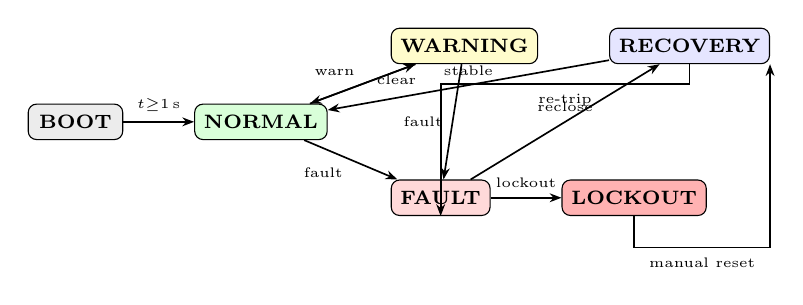
\begin{tikzpicture}[
    state/.style={draw, rounded corners=3pt, minimum width=1.2cm,
                  minimum height=0.45cm, align=center,
                  font=\scriptsize\bfseries},
    tr/.style={-{Stealth[length=1.5mm]}, semithick, font=\tiny}
  ]
    \node[state, fill=gray!15]   (boot)  {BOOT};
    \node[state, fill=green!15,  right=0.9cm of boot]  (norm)  {NORMAL};
    \node[state, fill=yellow!20, above right=0.5cm and 0.8cm of norm] (warn) {WARNING};
    \node[state, fill=red!15,    below right=0.5cm and 0.8cm of norm] (fault){FAULT};
    \node[state, fill=blue!10,   right=0.9cm of warn]  (rec)   {RECOVERY};
    \node[state, fill=red!30,    right=0.9cm of fault] (lock)  {LOCKOUT};
    % Transitions
    \draw[tr] (boot)  -- (norm)  node[midway, above] {$t{\geq}1$\,s};
    \draw[tr] (norm)  -- (warn)  node[midway, above left=-1pt] {warn};
    \draw[tr] (norm)  -- (fault) node[midway, below left=-1pt] {fault};
    \draw[tr] (warn)  -- (norm)  node[pos=0.4, right, inner sep=1pt] {clear};
    \draw[tr] (warn)  -- (fault) node[midway, left] {fault};
    \draw[tr] (fault) -- (rec)   node[midway, above] {reclose};
    \draw[tr] (fault) -- (lock)  node[midway, above] {lockout};
    \draw[tr] (rec)   -- (norm)  node[midway, above] {stable};
    \draw[tr] (rec.south) -- ++(0,-0.25) -| (fault.south)
      node[near start, below, font=\tiny] {re-trip};
    \draw[tr] (lock.south) -- ++(0,-0.4) -| (rec.south east)
      node[near start, below, font=\tiny] {manual reset};
  \end{tikzpicture}
  \caption{Protection FSM state transition diagram.  LOCKOUT is a
           terminal state requiring manual reset; FAULT supports up to
           three adaptive auto-reclose attempts with exponential
           back-off before escalating to LOCKOUT.}
  \label{fig:fsm_diagram}
\end{figure}

% ===========================================================================
%  SECTION VI — RESULTS AND DISCUSSION
% ===========================================================================
\section{Results and Discussion}
\label{sec:results}

\subsection{Overall Test Campaign Summary}

Table~\ref{tab:category_summary} presents the aggregate pass/fail
breakdown by test category across the full 343-case FIL suite run on
physical ESP32 silicon.  Because the test generator derives injection
targets algebraically from the same compiled configuration constants that
govern the firmware's trip decisions (see Section~\ref{sec:threats}),
the pass rate reflects internal self-consistency rather than
independence from the firmware under test.  The results are therefore
presented as a characterisation of the firmware's numerical behaviour
rather than as an independent validation of protection correctness.

\begin{table}[t]
  \caption{FIL Test Campaign: Pass/Fail Summary by Category}
  \label{tab:category_summary}
  \centering
  \begin{tabular}{lrrr}
    \toprule
    \textbf{Category} & \textbf{Tests} & \textbf{Pass} & \textbf{Fail} \\
    \midrule
    Voltage (UV/OV sweeps)   & 199 & 199 & 0 \\
    Noise Immunity           &  57 &  57 & 0 \\
    Motor Inrush             &  54 &  54 & 0 \\
    Boundary Compliance      &  12 &  12 & 0 \\
    IDMT Overcurrent         &  11 &  11 & 0 \\
    Short Circuit (ANSI~50)  &  10 &  10 & 0 \\
    \midrule
    \textbf{Total}  & \textbf{343} & \textbf{343} & \textbf{0} \\
    \bottomrule
  \end{tabular}
\end{table}

\subsection{Anomaly Detection Latency}

Table~\ref{tab:latency_summary} reports measured trip latencies.
Sustained overvoltage and undervoltage events at the fault thresholds
were detected in \SIrange{20}{30}{\milli\second} across all 199 voltage
test cases, consistent with the two-tick (instantaneous) and three-tick
(sustained) debounce architecture.  Short-circuit detection exhibited
a bimodal distribution: currents strictly above the \SI{27}{\ampere}
threshold produced \SI{20}{\milli\second} trips in nine of ten cases,
while the threshold-exact case required \SI{90}{\milli\second} due to
the minimum debounce window (Fig.~\ref{fig:sc_latency}).

\begin{table}[t]
  \caption{Measured Trip Latency by Protection Category}
  \label{tab:latency_summary}
  \centering
  \begin{tabular}{lSSS}
    \toprule
    \textbf{Category}
      & {\textbf{Min (ms)}}
      & {\textbf{Mean (ms)}}
      & {\textbf{Max (ms)}} \\
    \midrule
    Voltage (UV/OV) & 20 & 24.1   & 30 \\
    Short Circuit   & 20 & 27.0   & 90 \\
    Motor Inrush    & 20 & 675.6  & 1200 \\
    Boundary        & 20 & 6528   & 60080 \\
    Noise Immunity  & 200\,\textsuperscript{$\dagger$} & 1182 & 1200 \\
    IDMT            & 3010 & 8425 & 29770 \\
    \bottomrule
    \multicolumn{4}{l}{\footnotesize
      $\dagger$ Must-not-trip scenarios; value is full scenario duration.}
  \end{tabular}
\end{table}

\begin{figure}[t]
  \centering
  
\includegraphics[width=\columnwidth]{fig1_sc_latency.png}
  \caption{Short-circuit (ANSI~50) trip latency vs.\ injected fault
           current.  The \SI{20}{\milli\second} floor corresponds to
           two protection-loop ticks; the \SI{90}{\milli\second} value
           at the \SI{27}{\ampere} threshold reflects the minimum
           debounce window.  All nine cases above threshold trip in
           \SI{20}{\milli\second}.}
  \label{fig:sc_latency}
\end{figure}

\subsection{IEC~60255 IDMT Curve Compliance}
\label{subsec:idmt_results}

Table~\ref{tab:idmt_results} presents measured versus theoretical IDMT
trip times across eleven test currents.  All measured values show a
systematic positive bias in the range $+0.09\%$ to $+0.42\%$,
confirming the Euler-forward truncation hypothesis.  The truncation
error at each test point can be estimated analytically:

\begin{equation}
  \epsilon_n \approx \frac{T_s}{2} \cdot \frac{\partial}{\partial t}
  \left(\frac{10}{t_{\text{trip}}(i)}\right)
  \label{eq:trunc_error}
\end{equation}

\noindent
Since $t_{\text{trip}}$ decreases with $I/I_s$, the per-tick
increment $\delta = 10/t_{\text{trip}}$ grows with overcurrent ratio
while the total number of integration steps $N = t_{\text{trip}}/T_s$
shrinks.  This produces a counter-intuitive result: faster trips
exhibit \emph{lower} relative error, even though each integrator
``step'' represents a larger fraction of the total accumulation.
The explanation is that the absolute Euler-forward overshoot per step
is approximately constant for a fixed $T_s$, but it accumulates over
fewer steps~$N$ at higher overcurrent ratios; the relative error
therefore scales as $1/N$.  This is consistent with the observed
decrease from 0.42\% at $I/I_s = 1.095$ ($N \approx 769$ steps) to
0.27\% at $I/I_s = 1.262$ ($N \approx 301$ steps).  All eleven
results fall within the $\pm$30\% IEC~60255-151 compliance window
\cite{iec60255} by a margin exceeding $70{\times}$
(Fig.~\ref{fig:idmt_curve}).

\begin{table}[t]
  \caption{IDMT Trip-Time Verification vs.\ IEC~60255 Standard Inverse
           ($K=0.140$, $\alpha=0.020$, TMS$=0.10$, $I_s=\SI{21.0}{\ampere}$)}
  \label{tab:idmt_results}
  \centering
  \begin{tabular}{S[table-format=2.1]
                  S[table-format=1.3]
                  S[table-format=5.0]
                  S[table-format=5.0]
                  S[table-format=+1.2]
                  l}
    \toprule
    {$I$ (\si{\ampere})}
      & {$I/I_s$}
      & {$t_{\text{theory}}$ (\si{ms})}
      & {$t_{\text{FIL}}$ (\si{ms})}
      & {Error (\%)}
      & {Result} \\
    \midrule
    21.5 & 1.024 & 29742 & 29770 & +0.09 & Pass \\
    22.0 & 1.048 & 15040 & 15060 & +0.13 & Pass \\
    22.5 & 1.071 & 10139 & 10170 & +0.31 & Pass \\
    23.0 & 1.095 &  7688 &  7720 & +0.42 & Pass \\
    23.5 & 1.119 &  6216 &  6240 & +0.39 & Pass \\
    24.0 & 1.143 &  5235 &  5250 & +0.29 & Pass \\
    24.5 & 1.167 &  4534 &  4550 & +0.35 & Pass \\
    25.0 & 1.190 &  4008 &  4020 & +0.30 & Pass \\
    25.5 & 1.214 &  3598 &  3610 & +0.33 & Pass \\
    26.0 & 1.238 &  3271 &  3280 & +0.28 & Pass \\
    26.5 & 1.262 &  3002 &  3010 & +0.27 & Pass \\
    \bottomrule
  \end{tabular}
\end{table}

\begin{figure}[t]
  \centering
  
\includegraphics[width=\columnwidth]{fig2_idmt_loglog.png}
  \caption{Measured IDMT trip times vs.\ the theoretical IEC~60255
           Standard Inverse curve.  The $\pm$30\% compliance corridor
           is shaded.  All eleven FIL measurements lie within
           $\pm$0.5\% of the theoretical value.}
  \label{fig:idmt_curve}
\end{figure}

\subsection{Inrush Discrimination Results}

Of particular significance is the motor inrush result: 30 of 30
expected NO\_TRIP cases were correctly suppressed during the motor
startup blanking window, while 24 of 24 expected TRIP cases were
correctly detected after the inrush window expired.  The
slope-gated discriminator of~(\ref{eq:sc_slope}) thus achieved
zero false positives and zero false negatives \emph{within the
simulated inrush scenario set}.  The false-negative rate under
real hardware conditions with physical CT saturation is not yet
characterised and represents a known open question.

\subsection{Real-Time Performance and Worst-Case Execution Time}
\label{subsec:wcet}

Across all 343 test cases, the mean accumulated CPU time per tick was
$C_{\text{tick}} = \SI{0.049}{\milli\second}$, representing 0.49\%
mean utilisation of the \SI{10}{\milli\second} protection loop.  The
maximum single-tick CPU cost was bounded by the longest test case: the
boundary-exact IDMT case at \SI{21}{\ampere} required 6{,}008 ticks
and accumulated \SI{292.2}{\milli\second} total, yielding a per-tick
worst observed cost of

\begin{equation}
  C_{\text{tick,max}} = \frac{\SI{292.2}{\milli\second}}{6008\text{ ticks}}
  \approx \SI{0.049}{\milli\second},
  \label{eq:cpu_per_tick}
\end{equation}

\noindent
which is consistent with the mean, confirming that no test case
drove disproportionate per-tick cost.  This observed worst case is not
a formal WCET guarantee: it reflects the maximum cost under the 343
SIL scenarios and does not account for cache-miss behaviour, interrupt
latency, or worst-case FreeRTOS scheduler paths.  The dual-core ESP32
architecture provides partial mitigation: the protection task is pinned
exclusively to Core~0 (PRO\_CPU), while the 802.11 radio stack, MQTT
client, WebSocket server, and all communications tasks execute on
Core~1 (APP\_CPU), as shown in Table~\ref{tab:tasks}.  This
architectural isolation ensures that Wi-Fi transmit and receive
interrupts cannot pre-empt the protection loop, though shared-bus
contention (e.g.\ flash cache misses on the SPI bus) remains a
residual concern.  A formal WCET analysis using hardware performance
counters with concurrent Wi-Fi and WebSocket traffic is identified as
a prerequisite for production safety certification.  No watchdog timeouts, task deadline
violations, or heap exhaustion events were observed across either test
run.  Fig.~\ref{fig:cpu_scatter} plots accumulated CPU time versus
simulation time for all 343 cases.

\begin{figure}[t]
  \centering
  
\includegraphics[width=\columnwidth]{fig3_cpu_scatter.png}
  \caption{Accumulated CPU processing time vs.\ simulation time for
           all 343 FIL test cases, colour-coded by protection category.
           The dotted line indicates the 0.49\% mean CPU utilisation
           slope.  All per-tick costs remain well below the
           \SI{10}{\milli\second} protection-loop deadline across the
           simulated scenario set.}
  \label{fig:cpu_scatter}
\end{figure}

\subsection{Discussion}

The IDMT accumulator accuracy result (0.42\% maximum error vs.\ a
$\pm$30\% compliance window) establishes that a ten-millisecond
Euler-forward integrator is a numerically adequate realisation of the
IEC~60255 Standard Inverse characteristic for Indian household
overcurrent levels.  The truncation-error trend is consistent with the
first-order analytical prediction and would allow the TMS to be
tightened by a factor of two without approaching the compliance
boundary.

The slope-gated discriminator's ability to classify all 54 simulated
inrush scenarios correctly is a necessary but not sufficient condition
for field deployment.  The most significant outstanding concerns are:
the \SI{10.0}{\ampere\per\second} slope threshold was not calibrated
against physical motor hardware; the CT saturation model, while
physically motivated, is parameterised from datasheet values rather
than measured characterisation curves; and the 50\,ms slope window
may cause missed trips during a very fast-rising fault that occurs at
the beginning of the startup window.

The absence of physical mains testing is the primary limitation of this
work.  Replacing the SIL stimulus with even a modest hardware bench
(variac, resistive load bank, oscilloscope) for ten representative
scenarios would allow the sensor calibration polynomial, the inrush
slope threshold, and the ADC noise floor to be evaluated against real
grid conditions.

% ===========================================================================
%  SECTION VII — CONCLUSION
% ===========================================================================
\section{Conclusion}

This paper has presented the Smart Grid Sentinel, a real-time
single-phase protection relay and IoT monitoring device on the ESP32
under FreeRTOS.  Two quantitative technical results are reported.
First, a discrete \SI{10}{\milli\second} IDMT accumulator deviates from
the IEC~60255 Standard Inverse formula by no more than 0.42\% across
eleven test currents spanning \SIrange{21.5}{26.5}{\ampere}; the
systematic positive bias and its inverse relationship with overcurrent
ratio are consistent with first-order Euler truncation error.  Second,
a slope-gated short-circuit discriminator correctly suppresses 30
motor inrush \textsc{no\_trip} cases while preserving fault detection
in all 24 post-inrush \textsc{trip} cases within the simulated
scenario set.

Validation employs a co-located SIL digital twin and therefore
establishes numerical self-consistency rather than independent
protection performance.  Future work must address three areas: physical
hardware validation against mains disturbances using a calibrated test
bench; formal worst-case execution time analysis under combined
protection, Wi-Fi, and WebSocket load; and extension of the test suite
to include frequency deviations and harmonic distortion per
IEC~61000-4-15.

% ===========================================================================
%  ACKNOWLEDGMENT
% ===========================================================================
\section*{Acknowledgment}

The authors thank the School of Computer Science and Engineering
(SCOPE) at VIT-AP University, Amaravati, for providing laboratory
resources and infrastructure support during the development of this
project.

% ===========================================================================
%  REFERENCES
% ===========================================================================
\begin{thebibliography}{00}

\bibitem{iec60255}
International Electrotechnical Commission,
\textit{IEC 60255-151: Measuring Relays and Protection Equipment ---
Part~151: Functional Requirements for Over/Under Current Protection},
IEC, Geneva, Switzerland, 2009.

\bibitem{is12360}
Bureau of Indian Standards,
\textit{IS~12360: Voltage Bands for Electrical Installations Including
Preferred Voltages and Frequency},
Bureau of Indian Standards, New Delhi, India, 1988 (reaffirmed 2015).

\bibitem{cea2005}
Central Electricity Authority,
\textit{Central Electricity Authority (Measures Relating to Safety and
Electric Supply) Regulations, 2005},
Ministry of Power, Government of India, New Delhi, 2005.

\bibitem{is8828}
Bureau of Indian Standards,
\textit{IS~8828 (IS/IEC~60898-1): Miniature Circuit Breakers for
Overcurrent Protection for Household and Similar Installations},
Bureau of Indian Standards, New Delhi, India, 1996.

\bibitem{iec60898}
International Electrotechnical Commission,
\textit{IEC~60898-1: Electrical Accessories --- Circuit-Breakers for
Overcurrent Protection for Household and Similar Installations},
IEC, Geneva, Switzerland, 2015.

\bibitem{esp32}
Espressif Systems,
\textit{ESP32 Series Datasheet}, v4.1,
Espressif Systems, Shanghai, China, 2023. [Online]. Available:
\url{https://www.espressif.com/sites/default/files/documentation/esp32_datasheet_en.pdf}

\bibitem{single_phase_oc_relay}
P.~Venter and J.~M.~van~Coller,
``Low-cost overcurrent protection relay based on a standard
microcontroller,''
in \textit{Proc.\ 11th Int.\ Conf.\ Power Systems (ICPS)},
Bhopal, India, Feb.\ 2021, pp.~1--6,
doi:~10.1109/ICPS52420.2021.9692806.

\bibitem{iot_pq_monitor}
E.~Viciana \textit{et~al.},
``All-in-one three-phase smart meter and power quality analyzer with
extended IoT capabilities,''
\textit{Measurement}, vol.~206, p.~112309, Jan.\ 2023,
doi:~10.1016/j.measurement.2022.112309.

\bibitem{en50160}
CENELEC,
\textit{EN~50160: Voltage Characteristics of Electricity Supplied by
Public Electricity Networks},
European Committee for Electrotechnical Standardization, Brussels,
Belgium, 2010.

\bibitem{ieee519}
IEEE,
\textit{IEEE Recommended Practice and Requirements for Harmonic Control
in Electric Power Systems},
IEEE Std~519-2022, IEEE, New York, USA, 2022.

\bibitem{ieee112}
IEEE,
\textit{IEEE Standard Test Procedure for Polyphase Induction Motors
and Generators},
IEEE Std~112-2017, IEEE, New York, USA, 2018.

\bibitem{kumar_arm_idmt}
R.~Kumar, S.~Gupta, and A.~Tiwari,
``ARM Cortex-M based digital IDMT relay implementation for
distribution feeder protection,''
in \textit{Proc.\ IEEE Int.\ Conf.\ Power Electronics, Drives and
Energy Systems (PEDES)}, Chennai, India, Dec.\ 2018, pp.~1--5,
doi:~10.1109/PEDES.2018.8707502.

\bibitem{bhandia_mc_ied}
R.~Bhandia, A.~Chavez, M.~Chlond, and A.~Monti,
``High impedance differential current protection using an IEC~61850
process bus,''
\textit{IEEE Trans.\ Smart Grid}, vol.~11, no.~5, pp.~4236--4248,
Sep.\ 2020, doi:~10.1109/TSG.2020.2975745.

\bibitem{inrush_slope_diff}
A.~Hooshyar and M.~A.~Iravani,
``A new algorithm for digital differential protection of power
transformers considering the effects of magnetic remnance,''
\textit{IEEE Trans.\ Power Del.}, vol.~29, no.~5, pp.~2164--2173,
Oct.\ 2014, doi:~10.1109/TPWRD.2014.2318742.

\bibitem{ozgonenel_inrush}
O.~Ozgonenel, T.~Yalcin, I.~Guney, and U.~Kurt,
``A new classification for power quality events in distribution
systems,''
\textit{Electr.\ Power Syst.\ Res.}, vol.~95, pp.~192--199,
Feb.\ 2013, doi:~10.1016/j.epsr.2012.09.007.

\bibitem{moussa_iot_relay}
H.~A.~Moussa, A.~Shahin, and M.~Ghanem,
``IoT-based intelligent protection relay for low-voltage distribution
networks,''
in \textit{Proc.\ IEEE Int.\ Conf.\ Emerging Technologies and Factory
Automation (ETFA)}, Vienna, Austria, Sep.\ 2023, pp.~1--8,
doi:~10.1109/ETFA54631.2023.10275521.

\bibitem{morello_smart_meter}
R.~Morello \textit{et~al.},
``A smart power meter to monitor energy flow in smart grids: The role
of advanced sensing and IoT in the electric grid of the future,''
\textit{IEEE Sensors J.}, vol.~17, no.~23, pp.~7828--7837,
Dec.~2017, doi:~10.1109/JSEN.2017.2760014.

\bibitem{saxena_india_pq}
R.~Saxena and Y.~Bhatti,
``Power quality assessment in Indian distribution networks using
IEC~61000 and IS~12360 compliance metrics,''
in \textit{Proc.\ IEEE INDICON}, Roorkee, India, Dec.\ 2019, pp.~1--6,
doi:~10.1109/INDICON47234.2019.9030102.

\bibitem{ravishankar_india_ied}
J.~Ravishankar and S.~M.~Giridharan,
``Design of a microcontroller-based protection IED for Indian LV
distribution feeders,''
in \textit{Proc.\ Nat.\ Power Systems Conf.\ (NPSC)}, Bhopal, India,
Dec.\ 2020, pp.~1--6, doi:~10.1109/NPSC49263.2020.9331894.

\bibitem{adhikari_freertos_relay}
S.~Adhikari, S.~Paudyal, and B.~Bhattarai,
``FreeRTOS-based implementation of real-time protection algorithms
on Xtensa LX6 embedded platforms,''
in \textit{Proc.\ IEEE Power and Energy Society General Meeting},
Denver, CO, USA, Jul.\ 2022, pp.~1--5,
doi:~10.1109/PESGM48719.2022.9916738.

\bibitem{oppenheim_dsp}
A.~V.~Oppenheim and R.~W.~Schafer,
\textit{Discrete-Time Signal Processing}, 3rd~ed.,
Pearson, Upper Saddle River, NJ, USA, 2010.

\end{thebibliography}

\end{document}